One lasting scientific legacy of the {\it Hubble Space Telescope
(HST)} will be the discovery of giant black holes at the centers of
galaxies, confirming the longstanding theory of the ``central
engines'' of quasars.  One of the major surprises from the {\it
Hubble} was the discovery of a correlation between black hole mass and
host galaxy properties.\footnote{Assessment of Options for Extending
the Life of the Hubble Space Telescope: Final Report (2005);
https://www.nap.edu/read/11169/chapter/5).}  This connection, causal
or otherwise, may provide crucial clues to how and why these black
holes formed and how their host galaxies evolved. {\it As of the
launch of the James Webb Space Telescope (JWST), the question of how
black holes affect their host galaxies is one of the outstanding
questions in astrophysics.}

\smallskip \smallskip
\noindent
Observational and theoretical work now suggests that active galaxies
and black holes are potentially linked to both the triggering, and
``quenching'', of massive star formation. The link between massive
galaxies and the central super-massive black holes (SMBHs) that seem
ubiquitous in them is now thought to be vital to the understanding of
galaxy formation and evolution ([1], [2]), and huge observational and
theoretical effort has been invested in trying to measure and
understand the physics involved in these enigmatic systems.  The two
main energy sources available to a galaxy are nuclear fusion in stars
and gravitational accretion onto compact objects, and we still do not
fully understand the interaction of an active galactic nuclei and the
star formation properties of their host galaxies, {\it especially at
the epoch of maximal cosmic SFR and quasar activity, redshifts $z\sim1-3$.}

\smallskip \smallskip
\noindent
The ``quenching'' of galaxy-wide star formation, is supposedly driven
by `` AGN feedback'', where the AGN helps to heat the surrounding gas
corona, offsetting cooling losses and disrupting the gas inflow. This
feedback manifests itself as high-velocity outflows from the
AGN/quasar.  However, {\it direct observational evidence} for AGN
feedback is conspicuous by its absence. This is especially true at
high-$z$, e.g. $z=2-3$, at the height of the Quasar Epoch.  We have
identified the best candidates that suggest we are seeing quasar
feedback in action, in situ at high-redshift. These are the
``Extremely Red Quasars'' identified via their WISE W3/4 colors.  As
such, these mJy luminous AGN {\it are ideal targets for JWST
MIRI}.


\smallskip
\smallskip
\noindent
{\bf \underline{The Extremely Red Quasar Population}:} By matching the
quasar catalogues of the Sloan Digital Sky Survey (SDSS), the Baryon
Oscillation Spectroscopic Survey (BOSS) to the Wide-Field Infrared
Survey Explorer (WISE), Ross et al. (2015) discovered quasars with
extremely red infrared-to-optical colors: $r_{\rm AB}-W4_{\rm
Vega}>14$ mag, i.e., $F_\nu({\rm 22\mu m})/F_\nu(r) \gtrsim 1000$; see
Figure 1. These objects have infrared luminosities $\sim 10^{47}$ erg
s$^{-1}$.  The original motivation here was to look for PAHs that had
redshifted in the WISE W4 band for $z\approx2.5$ quasars in order to
study and link luminous AGN activity and star formation at the
``height of the quasar epoch''.

\smallskip
\smallskip
\noindent
Hamann et al. (2017) then fully and properly refined the selection of
the ERQs, homing the definition based on further analysis and common
properties, and indeed found many more objects in this new scheme. The
ERQs have a suite of peculiar emission-line properties including large
rest equivalent widths (REWs), unusual ``wingless'' line profiles,
large \nv /\lya , \nv /\civ , \siiv /\civ\ and other flux ratios, and
very broad and blueshifted [\oiii ] \lam 5007 (e.g. spectrum in
Figure~1).


\hspace{-7.5cm}
\begin{figure}[h]
  \begin{center}
    \hspace{-0.5cm}
    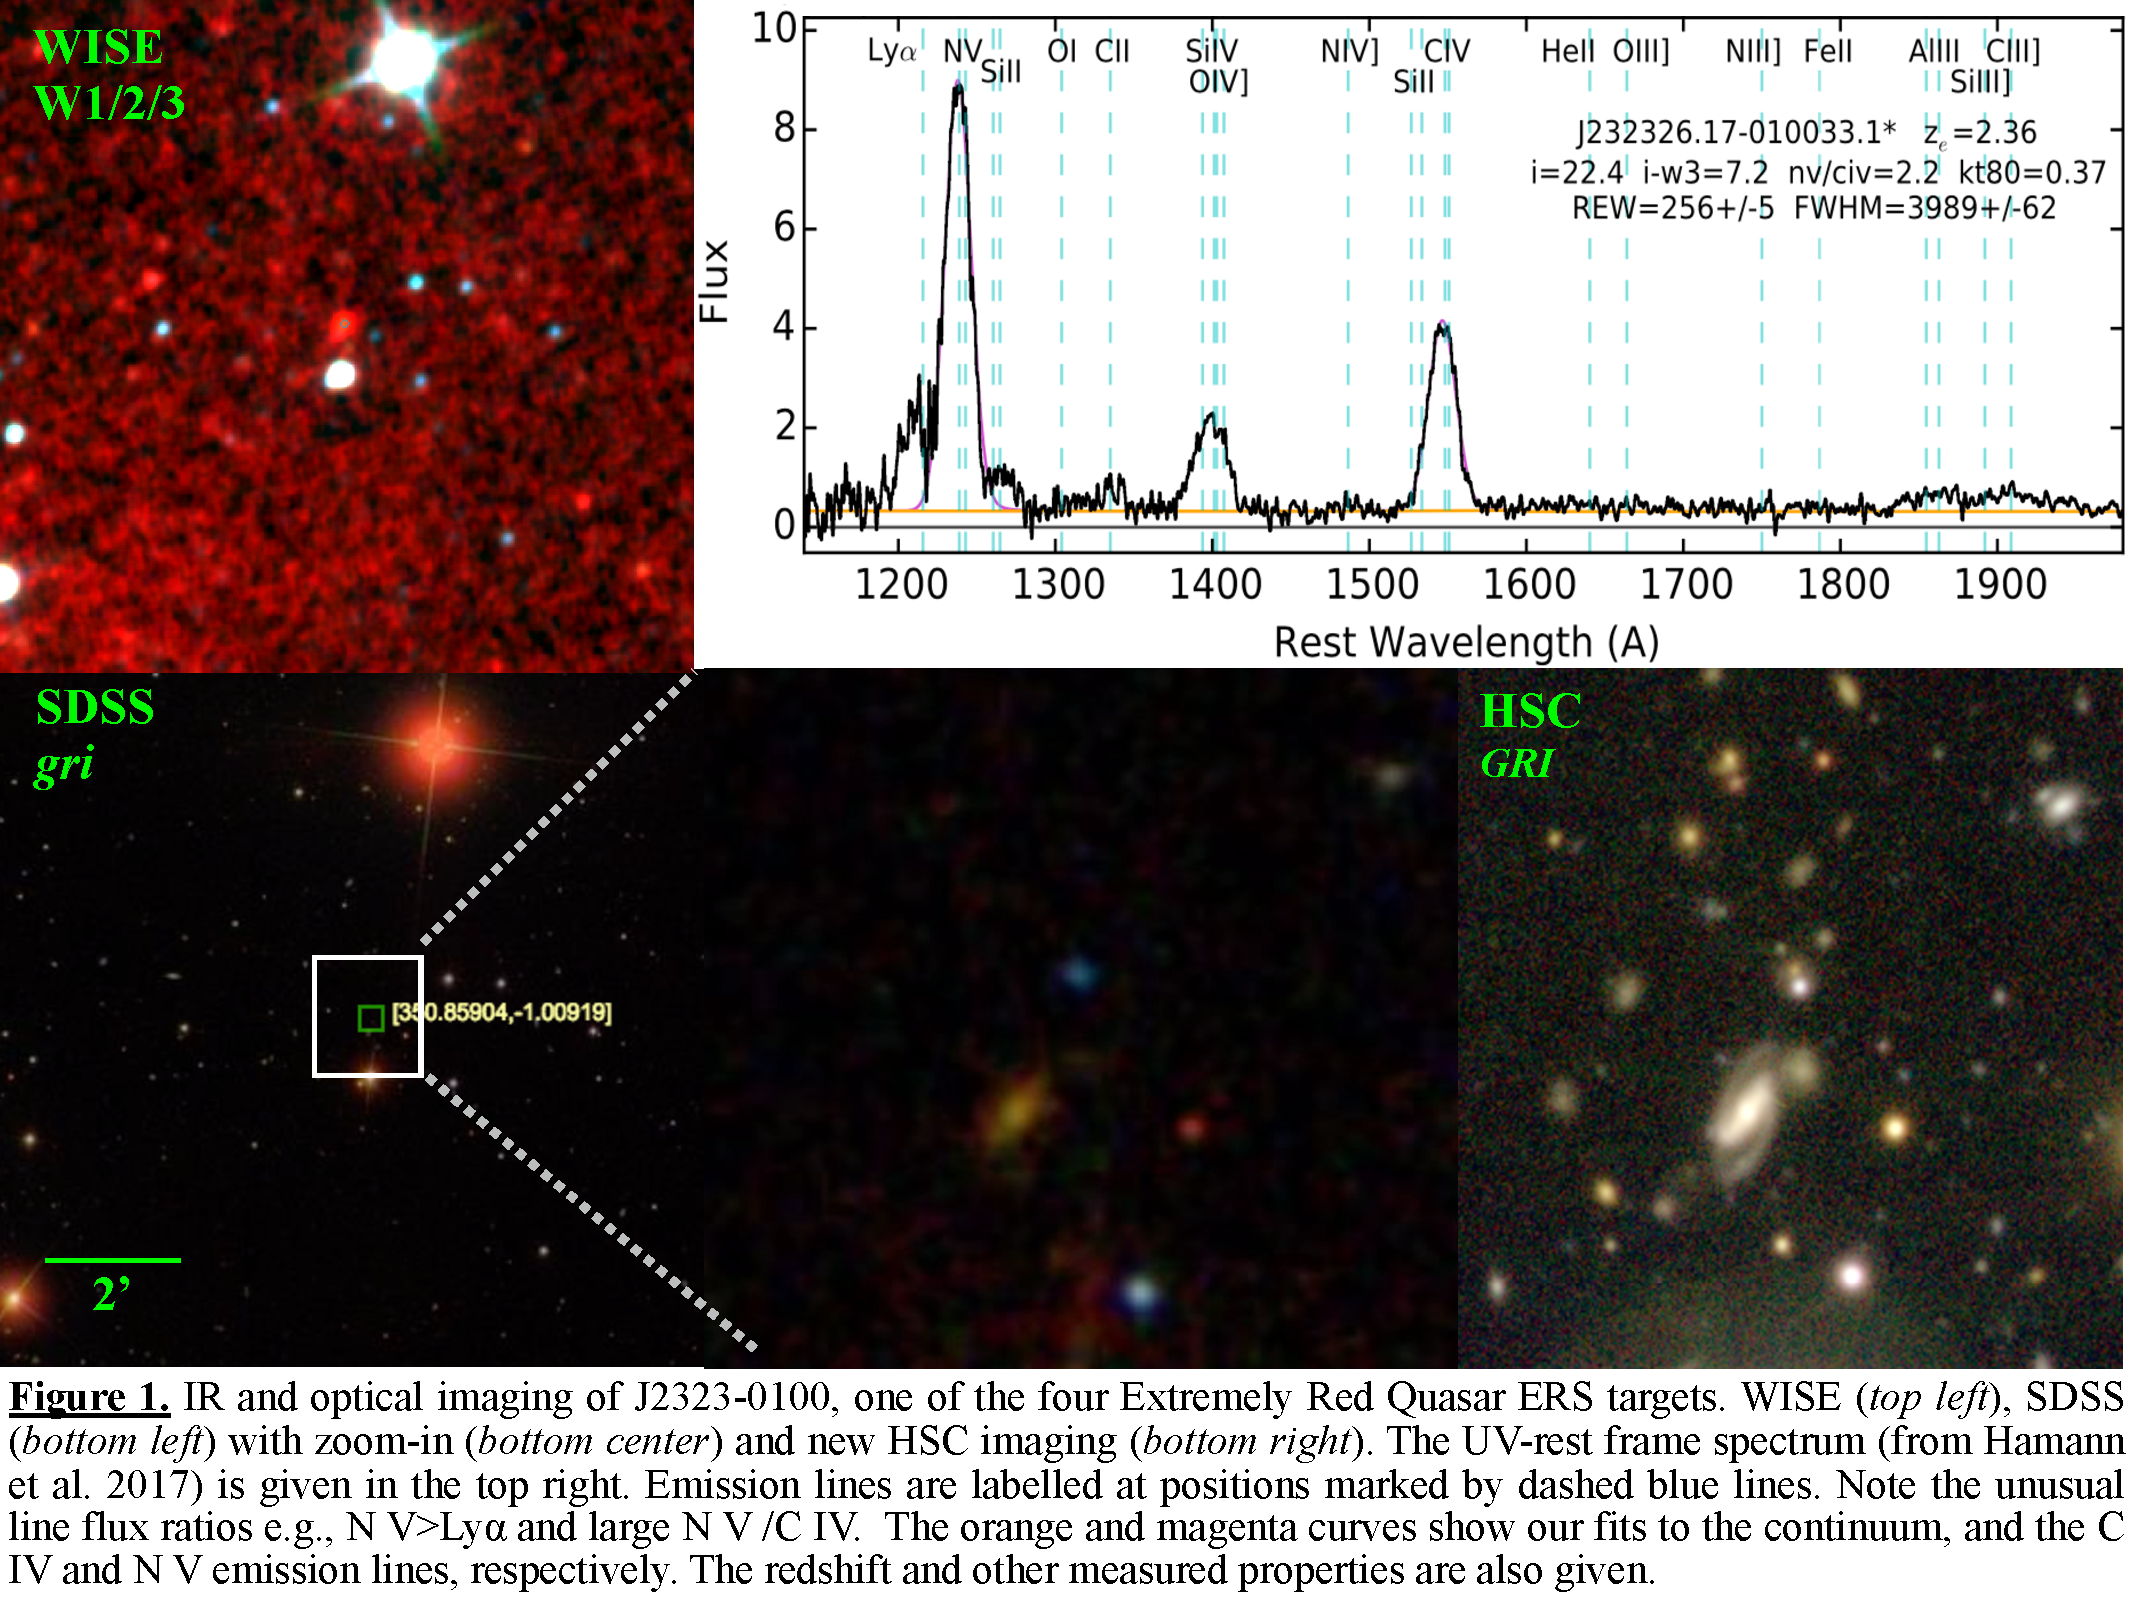
\includegraphics[height=12.0cm,width=16.0cm]{../Figures/WISE_SDSSzoomHSC_ERQ-image_v2.pdf}
%    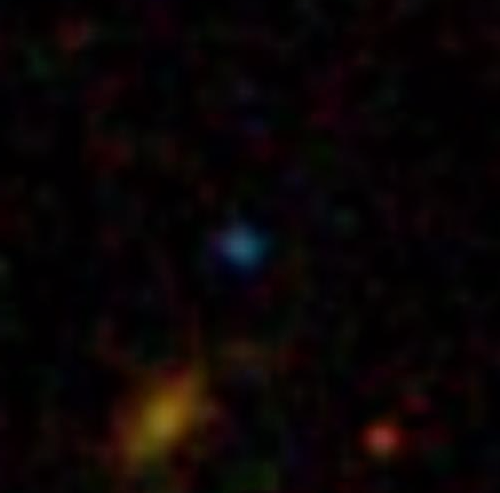
\includegraphics[height=6.0cm,width=6.0cm]{../Figures/ERQ_SDSS2_nolabel.png}
  %  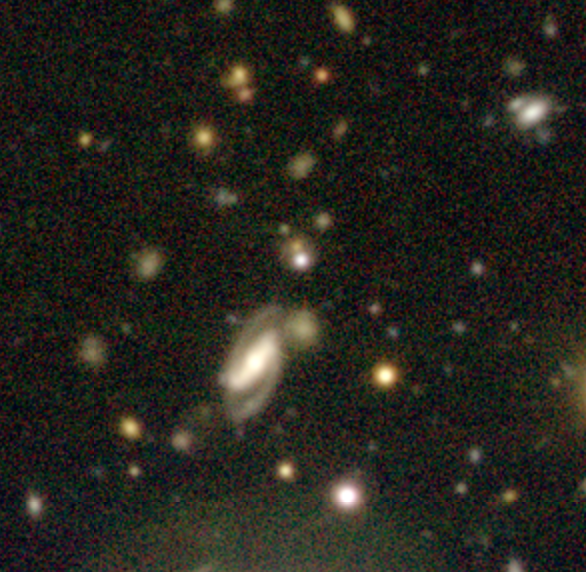
\includegraphics[height=6.0cm,width=6.0cm]{../Figures/ERQ_HSC1.png}
    %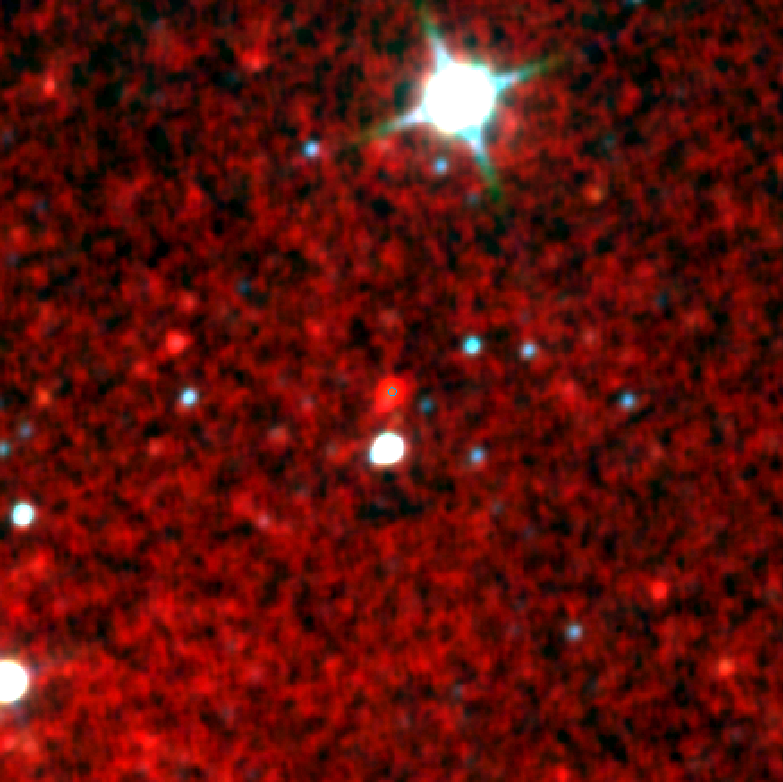
\includegraphics[height=6.0cm,width=6.0cm]{../Figures/ERQ_WISE_3band_v1.png}
    \vspace{-10pt}
%    \caption{
      % \small
%      \footnotesize
      % \scriptsize
      % \tiny
%      SDSS {\it (left)} and HSC {\it (right)} imaging of ERQ
 %     J2323-0100.  The gorgeous HSC data reveal a potential companion galaxy
  %    to J2323-0100 at the 11 o'clock position.
%}
    \vspace{-14pt}
    \label{figtest-fig}
  \end{center}
\end{figure}

\setcounter{figure}{1}
\hspace{-2.5cm}
\begin{figure}[h]
  \begin{center}
    \hspace{-0.5cm}
    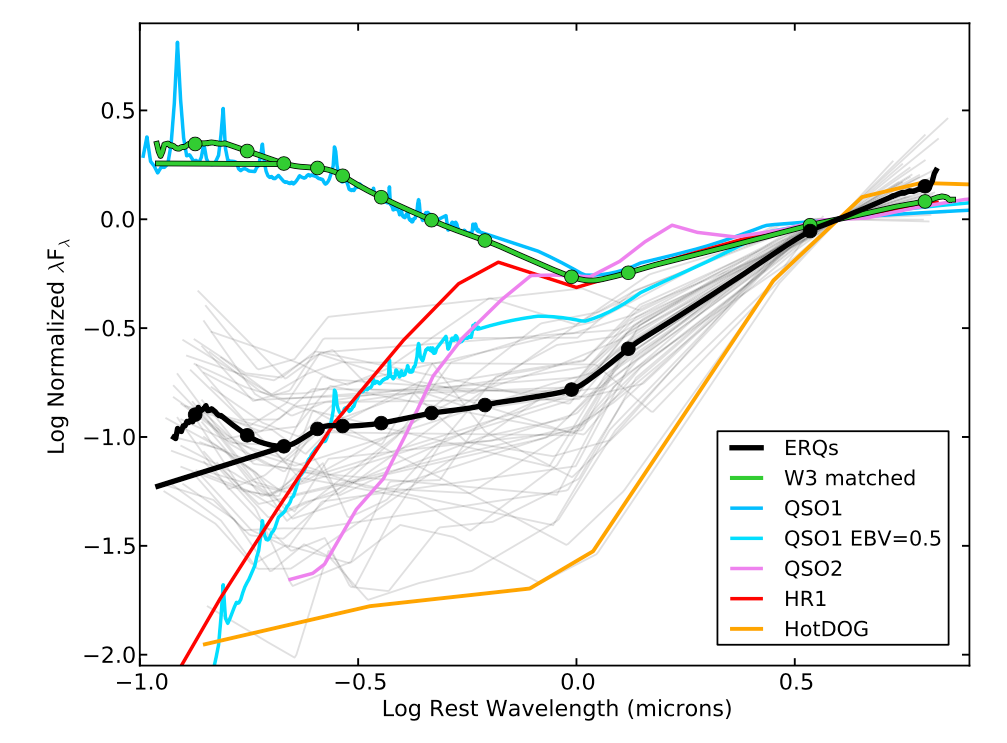
\includegraphics[height=7.0cm,width=7.0cm]{../Figures/Hamann2017_Fig16_SEDs.png}
    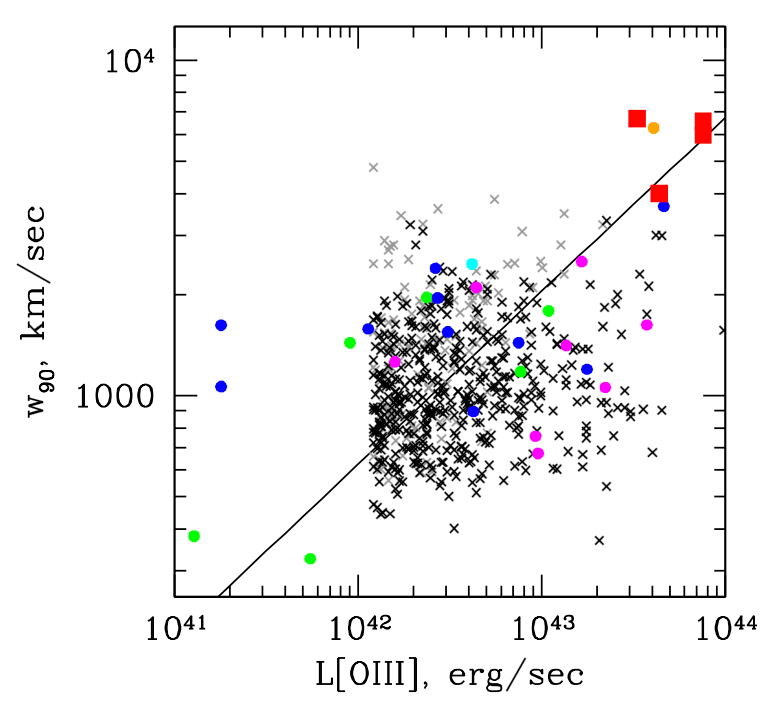
\includegraphics[height=7.1cm,width=7.4cm]{../Figures/Zakamska_2016_Fig9.png}
    \vspace{-10pt}
    \caption{
      % \small
      %\footnotesize
      \scriptsize
      % \tiny
      {\it (Left)} From Hamann et al., 2017, the normalized median
      SEDs for Type 1 non-BALs in the core ERQ sample (black curve) plus
      blue quasars matched to the core ERQs in W3 magnitude (green curve).
      The Type 1 quasar template with and without reddening equal to $E(B −
      V) = 0.5$ (light blue, `QSO1', from Polletta et al. 2007), a typical
      Type 2 quasar from Mateos et al. (2013; `QSO2', purple), a typical
      heavily reddened Type 1 quasar from Banerji et al. (2013; `HR1'), and
      a typical HotDOG from Tsai et al. (2015). The light grey curves are
      SEDs of individual core ERQs.
      %%
      {\it (Right)} \oiii\ kinematics as a function of luminosities
      for our four targets, red squares, with other quasar populations are
      shown by black points and various colored symbols.  At these extreme
      velocities, the gas cannot be confined by any realistic galaxy
      potential and is thus likely to escape from the galaxy; these objects
      are likely signposts of the extreme ‘blow-out’ phase of quasar
      feedback observed at the peak epoch of galaxy formation.
    }
    \vspace{-14pt}
    \label{fig:ERQ_SED}
  \end{center}
\end{figure}


\smallskip
\smallskip
\noindent
Our team identified a ``core'' sample of 97 ERQs with nearly uniform
peculiar properties selected via \imw\ $\ge 4.6$ (AB) and REW(\civ )
$\ge$ 100 \AA\ at redshifts 2.0--3.4.  The core ERQs have median
luminosity $\left<\log L ({\rm ergs/s})\right> \sim 47.1$, sky density
0.010 deg$^{-2}$, surprisingly flat/blue UV spectra given their red
UV-to-mid-IR colors, and common outflow signatures including BALs or
BAL-like features and large \civ\ emission-line blueshifts. Their
SEDs, see Figure~\ref{fig:ERQ_SED}, and line properties are
inconsistent with normal quasars behind a dust reddening
screen. Patchy obscuration by small dusty clouds could produce the
observed UV extinctions without substantial UV reddening.


\smallskip
\smallskip
\noindent
Further observations by our team with VLT-XShooter measured rest-frame
optical spectra of four $z\sim 2.5$ extremely red quasars (Zakamska et al. 2016).  
We discovered very broad (full width at half max$= 2600-5000$ km
s$^{-1}$), strongly blue-shifted (by up to 1500 km s$^{-1}$)
\oiii\ $\lambda$5007\AA\ emission lines in these objects. In a large
sample of type 2 and red quasars, \oiii\ kinematics are positively
correlated with infrared luminosity, and the four objects in our
sample are on the extreme end both in \oiii\ kinematics and infrared
luminosity.
%%
As such, we estimate that at least 3\% of the bolometric luminosity in
these objects is being converted into the kinetic power of the
observed wind. Photo-ionization estimates suggest that the \oiii
emission might be extended on a few kpc scales, which would suggest
that the extreme outflow is affecting the entire host galaxy of the
quasar.

\smallskip
\smallskip
\noindent
{\it We now believe that the core ERQs are a unique obscured quasar population
with extreme physical conditions related to powerful outflows across
the line-forming regions. These sources are the signposts of the most extreme form of
quasar feedback at the peak epoch of galaxy formation, and may
represent an active ``blow-out'' phase of quasar evolution. 
}


\medskip
\medskip
\smallskip
\smallskip
\noindent
{\bf \underline{MIR spectroscopy}:}
%% Fom Veilleux arXiv:0201118v1:: 
How do galaxies form? How do they evolve? How do supermassive black holes fit in this picture of galaxy formation? Which objects are the main contributors to the overall energy budget of the universe? To properly answer these questions, one needs to differentiate objects powered by nuclear fusion in stars (i.e. normal and starburst galaxies) from objects powered by mass accretion onto supermassive black holes (quasars and AGNs). A wide variety of diagnostic tools have been used in the past for this purpose with different degree of success.

\iffalse
Direct spectroscopy searches for the presence of the broad recombination lines at wavelengths where the effects of dust extinction are reduced.
We follow ``Veilleux's Commandments'':
\begin{itemize}
\item Thou shalt use lines which emphasize the differences between H II regions and AGNs; i.e., use high-ionization lines or low-ionization lines produced in the partially ionized zone. 
\item Thou shalt use strong lines which are easy to measure in typical spectra.
\item Thou shalt avoid lines which are badly blended with other emission or absorption line features.
\item Thou shalt use lines with small wavelength separation to minimize sensitivity to reddening.
\item Thou shalt use line ratios from the same elements or involving hydrogen recombination lines to eliminate or reduce abundance dependence.
\item Thou shalt avoid lines from Mg, Si, Ca, Fe – depleted onto dust grains. 
%\item Thou shalt use lines easily accessible to current UV/optical/IR detectors. 
\item Thou shalt avoid lines affected by strong stellar absorption features. 
\item Thou shalt avoid lines affected by strong atmospheric features.
\item Thou shalt use lines at long wavelengths to reduce the effects of dust extinction.
\end{itemize}
\fi

\smallskip
\smallskip
\noindent
%% {\bf From Padovani et al.,  arXiv:1707.07134v1}
%%3.4 MIR spectroscopy
IR spectroscopy, previously with the InfraRed Spectrograph (IRS;
Houck et al. 2004) on board the Spitzer Space Telescope, provided new
insights into the physics and classification of AGN. The unambiguous
observations of the silicate feature at 9.7 $\mu$m in emission in many
known AGN (Hao et al., 2005; Siebenmorgen et al., 2005; Sturm et al.,
2005; Buchanan et al., 2006; Shi et al., 2006) came as the long sought
confirmation of the unified scheme. At the same time, however, IRS
observations indicated that in some cases the source of obscuration
resides in the host rather than the torus (e.g. Goulding et al., 2012;
Hatziminaoglou et al., 2015).  
%%
Identification through MIR spectroscopy is very powerful, allowing to
detect obscured AGN components even when the MIR is dominated by the
host galaxy. Several classification diagrams have been developed to
determine the AGN contribution to an observed spectrum based on
certain spectral features, such as high ionisation emission lines like
\nev, \neii and \oiv, the EW of PAH features and the strength of the
silicate feature at 9.7 $\mu$m (see, e.g. Spoon et al., 2007; Armus et
al., 2007; Veilleux et al., 2009; Hernan-Caballero \& Hatziminaoglou,
2011). A number of techniques have also been developed to model the
observed MIR spectra and constrain the AGN and starburst contributions
(see e.g. Schweitzer et al., 2008; Nardini et al., 2008; Deo et al.,
2009; Feltre et al., 2013).

\smallskip
\smallskip
\noindent
Although MIR spectroscopy has had a great impact on our understanding
of AGN, the number of objects studied through these techniques is
limited when compared to photometric studies, as spectroscopic
observations require significantly longer integration
times. Ground-based observations are generally limited to the
brightest targets due to the effects of the Earth's atmosphere
(e.g. Alonso-Herrero et al., 2016), while medium deep observations were
only possible with the IRS during its cryogen-cooled phase. For the most
part, such observations were limited to $z\sim1$ luminous IR galaxies
(LIRGs), ultraluminous IR galaxies (ULIRGs), and a hand of Type 1 quasars
(Hernan-Caballero \& Hatziminaoglou, 2011, and references therein)
although a number of higher redshift ULIRGs were also studied by IRS
(see e.g. Kirkpatrick et al., 2012). 



\medskip
\medskip
\smallskip
\smallskip
\noindent
{\bf \underline{Polycyclic Aromatic Hydrocarbons}:}
Polycyclic Aromatic Hydrocarbons (PAHs) are abundant, ubiquitous, and
a dominant force in the interstellar medium of galaxies (see e.g.,
Tielens, 2008, ARAA, 46, 289 for a review).  Aromatic features are
already a significant component of dusty galaxy spectra as early as
$z\approx2$ (Yan et al., 2005, ApJ, 628, 604).  and the infrared (IR)
emission features at 3.3, 6.2, 7.7, 8.6, and 11.3 $\mu$m are generally
attributed to IR fluorescence from (mainly) far-ultraviolet (FUV)
pumped large polycyclic aromatic hydrocarbon (PAH) molecules. As such,
these features trace the FUV stellar flux and are thus a measure of
star formation (Peeters et al, 2004, ApJ, 613, 986).
%%
Given the redshift of our ERQs and the MIRI wavelength coverage we will coverage $1.36 \leq \lambda_{\rm emitted} \leq 8.6 \mu$m.




\section{Bibliography}
Fabian, 2012, ARAA 50, 455 $\bullet$ 
Kormendy \& Ho, 2013, ARAA, 51, 511 $\bullet$
Yuan \& Narayan, 2014, ARAA, 52, 529 $\bullet$
Heckman \& Best, 2014, ARAA, 52, 589  $\bullet$



\clearpage


